The main contribution of this thesis is represented by the design of a toolchain for Graph Neural Network acceleration on FPGA leveraging High-Level Synthesis.

This chapter explains in detail how the toolchain has been designed and how it can be used to build GNN accelerators to enhance inference performance.

The core component of the toolchain is the synthesizer, enclosing SODA-OPT~\cite{9786533} and PandA-Bambu~\cite{9586110}, upon which the research team responsible for supervising this thesis has dedicated significant efforts over the past years.
The primary objective of this thesis is to enhance SODA-OPT and Bambu to bridge GNN models written in high-level frameworks, such as PyTorch, to FPGA architectures.

Figure~\ref{fig:toolchain} illustrates the entire design flow, with the steps involved in the GNN acceleration process.
In particular, firstly, the GNN model is implemented in PyTorch, one of the most popular and powerful frameworks for Neural Network implementations.
Subsequently, the model is passed as input to Torch-MLIR, a crucial middle step that enables the generation of the MLIR representation.
This intermediate representation serves as input for the synthesizer, where, once the frontend optimization is complete, the refined version proceeds to the backend, where the actual GNN accelerator is effectively produced, ready to enhance inference performance on FPGA architectures.

The following Sections provide a comprehensive and in-depth exploration of each step within the proposed design flow.
This detailed breakdown highlights the various possibilities inherent in the toolchain and outlines the recommended procedures necessary to achieve the optimal outcome for GNN acceleration.
The thesis aims to equip researchers and practitioners in Graph Neural Networks with the necessary insights and understanding to harness the full potential of this toolchain and unleash the power of FPGA acceleration.

In conclusion, this thesis represents a significant advancement in Graph Neural Network acceleration.
By designing a refined toolchain and bridging the gap between high-level frameworks and FPGA architectures, this research contributes to the broader field of artificial intelligence.
It reinforces the potential of FPGA-based accelerators in revolutionizing the inference performance of GNN models.
The implications of this work offer a solid foundation for further exploration and advancements in the field of hardware acceleration for deep learning applications.

\begin{figure}[t]
    \centering
    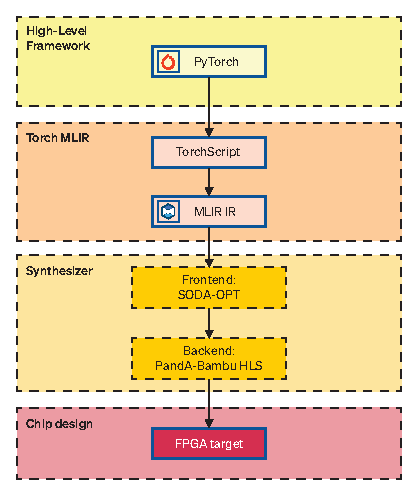
\includegraphics[height=0.6\textwidth]{Images/toolchain}
    \caption{FPGA Toolchain for Graph Neural Network Acceleration}
    \label{fig:toolchain}
\end{figure}

\section{PyTorch}
\label{sec:toolchain-pytorch}%

PyTorch~\cite{DBLP:journals/corr/abs-1912-01703} is an open-source deep learning framework widely used for building and training artificial neural networks for various machine learning tasks.

The first step of the toolchain is to design and implement the Graph Neural Network model in PyTorch.
Doing so involves defining the GNN model architecture and writing the necessary forward pass to compute node and graph-level representations.
Once having defined the model, the next step is training the GNN using standard PyTorch techniques, such as defining a loss function, setting up an optimizer, and performing backpropagation to optimize the model parameters.

\subsection{GNN models}
\label{subsec:gnn_models}%

Two main models have been used for this thesis: the Graph Isomorphism Network from OGB~\cite{NEURIPS2020_fb60d411, ogb_gnn_models}, written using PyTorch Geometric~\cite{DBLP:journals/corr/abs-1903-02428}, and the Graph Convolutional Network~\cite{DBLP:journals/corr/KipfW16, pygcn}, written using PyTorch~\cite{DBLP:journals/corr/abs-1912-01703}.

Most research and experiments have been conducted using the GCN model.
The GCN class, reported below, is characterized by two Graph Convolutional layers.

\begin{lstlisting}[language=Python,label={lst:gcn-class}]
import torch.nn as nn
import torch.nn.functional as F
from pygcn.layers import GraphConvolution

class GCN(nn.Module):
    def __init__(self, nfeat, nhid, nclass, dropout):
        super(GCN, self).__init__()

        self.gc1 = GraphConvolution(nfeat, nhid)
        self.gc1 = GraphConvolution(nhid, nclass)
        self.dropout = dropout

    def forward(self, x, adj):
        x = F.relu(self.gc1(x, adj))
        x = F.dropout(x, self.dropout, training=self.training)
        x = self.gc2(x, adj)
        return F.log_softmax(x, dim=1)
\end{lstlisting}

The forward function of each layer, reported below, is mainly characterized by two matrix multiplications.

\begin{lstlisting}[language=Python,label={lst:gcn-layer-forward}]

    def forward(self, input, adj):
        support = torch.mm(input, self.weight)
        output = torch.spmm(adj, support)
        if self.bias is not None:
            return output + self.bias
        else:
            return output
\end{lstlisting}

\subsection{Datasets}
\label{subsec:gnn_datasets}%

OGB provides different datasets that can be used with their models.
The one used for this thesis is called \textit{ogbg-molhiv}, a molecular property prediction dataset.
In each graph representing a molecule, nodes correspond to atoms, and edges represent chemical bonds.
The input node features consist of nine dimensions, encompassing information like atomic number, formal charge, and whether the atom is part of a ring.
The binary classification task consists in achieving precise predictions of target molecular properties, for example, determining whether a molecule inhibits HIV replication or not.

The dataset used for the GCN model is the \textit{Cora} one.
This dataset contains 2708 scientific publications, categorized into one of the seven classes considered.
The citation network contains 5429 links.
Each publication in the dataset is represented by a binary-valued word vector, indicating the absence or presence of the corresponding word from a dictionary of 1433 unique words.
The task is a multiclass classification, in which, given a paper, the objective is to classify it into one of the seven classes correctly.

\section{Torch-MLIR}
\label{sec:toolchain-torch_mlir}%

Torch-MLIR~\cite{torch_mlir} offers compiler support for transitioning from the PyTorch ecosystem to the MLIR ecosystem.

The steps Torch-MLIR follows to go from PyTorch to MLIR are shown in Figure~\ref{fig:torch-mlir}.
In particular, the flow followed in this thesis has been highlighted with blue arrows.
There are two starting points of the flow: TorchScript and LazyTensorCode.
The one used for this research, which is also the most tested one, is TorchScript.
TorchScript~\cite{torchscript} offers a way to generate serializable and optimizable models directly from PyTorch code.

The TorchScript representation is then converted to MLIR using the built-in conversion of Torch-MLIR. The result MLIR can use different dialects, but the one used for this thesis is the Linalg dialect, which serves as input for the next phase of the toolchain.

\begin{figure}[t]
    \centering
    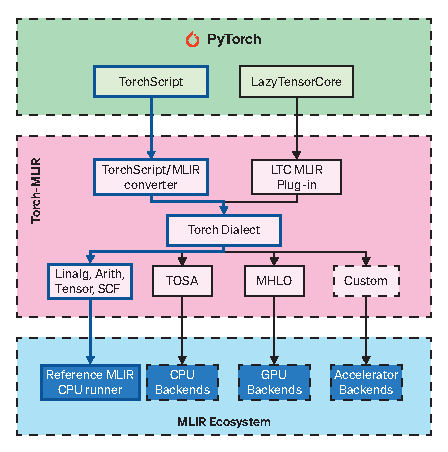
\includegraphics[height=0.5\textwidth]{Images/torch-mlir}
    \caption{Torch-MLIR flow}
    \label{fig:torch-mlir}
\end{figure}

\subsection{From PyTorch to TorchScript}
\label{subsec:pytorch-to-torchscript}%

\subsection{Torch-MLIR Compilation}
\label{subsec:torch-mlir-compilation}%

Once having designed, implemented, and trained the GNN model in PyTorch, it is possible to use the \texttt{torch\_mlir.compile} API to obtain the MLIR representation of the model.
This API takes three parameters as input, respectively:
\begin{enumerate}
    \item The Graph Neural Network model
    \item An input example of the model, the one that would be given for inference purposes
    \item The desired output type among the possible choices
\end{enumerate}

\section{Synthesizer}
\label{sec:toolchain-synthesizer}%

The synthesizer represents the final step of the toolchain, which optimizes and synthesizes the MLIR representation, targeting FPGA\@.
This step includes SODA-OPT and PandA-Bambu, both introduced in Section~\ref{sec:soda}.
The following Subsections provide insight into what is happening internally to these two components.

\begin{figure}[t]
    \centering
    \subfloat[Compiler frontend\label{fig:soda-opt_flow}]{
        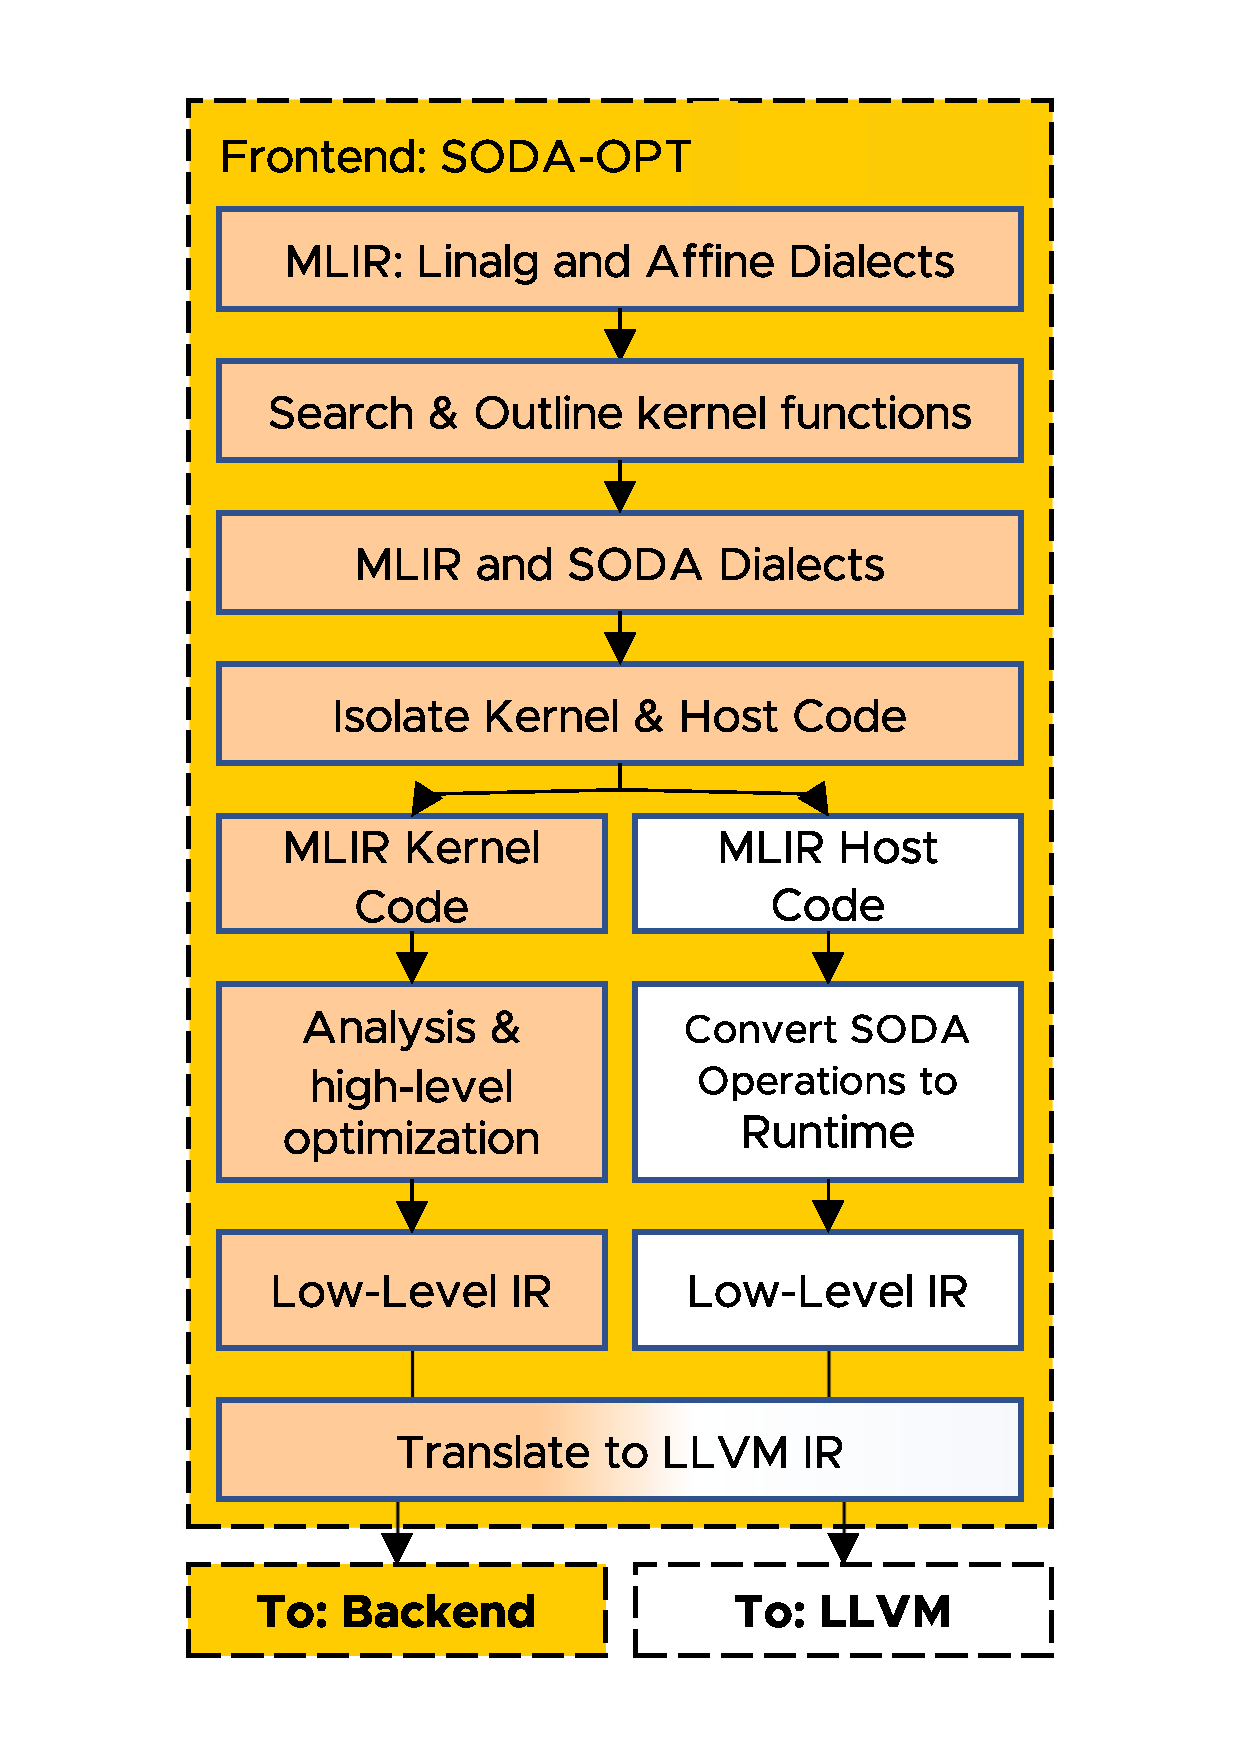
\includegraphics[height=0.5\textwidth]{Images/soda_opt_flow}
    }
    %\quad
    \hspace{0.03\textwidth}
    \subfloat[High-level synthesis backend\label{fig:bambu_flow}]{
        \captionsetup{width=.4\textwidth}
        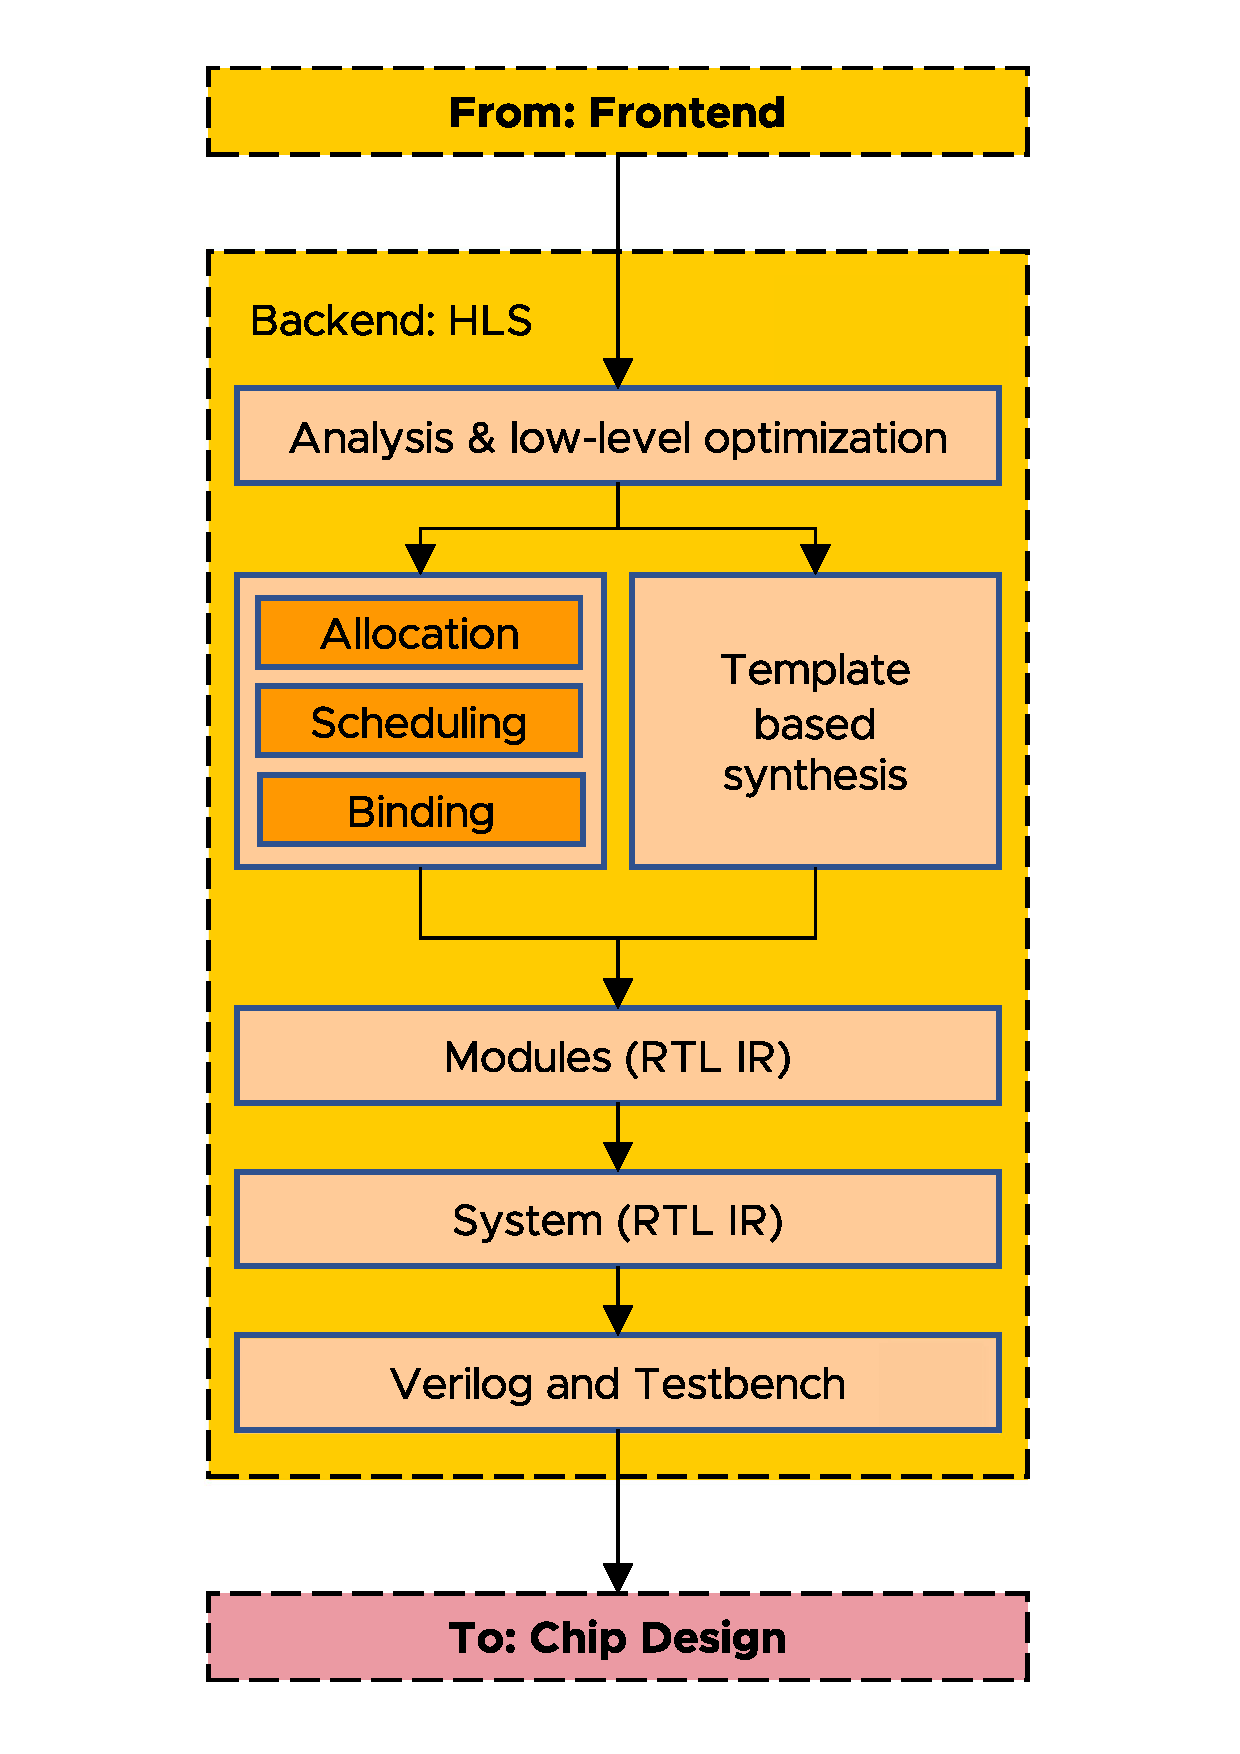
\includegraphics[height=0.5\textwidth]{Images/bambu_flow}
    }
    \caption{Synthesizer: SODA-OPT and PandA-Bambu overview~\cite{9786533}}
    \label{fig:synthesizer_flow}
\end{figure}

\subsection{SODA-OPT}
\label{subsec:toolchain-soda_opt}%

SODA-OPT, as shown in Figure~\ref{fig:soda-opt_flow}, receives as input the MLIR representation of the model, which must be modified by adding \texttt{soda.launch} and \texttt{soda.terminator} at the beginning and end of the piece of code that will be accelerated.

This step is primarily responsible for applying optimizations that can be exploited in the next step.
In particular, a subset of MLIR passes can be used to do so.
The output of SODA-OPT is an LLVM representation that serves as input to PandA-Bambu HLS\@.

\subsection{PandA-Bambu}
\label{subsec:toolchain-panda_bambu}%

PandA-Bambu represents the last phase of the synthesis.
As represented in Figure~\ref{fig:bambu_flow}, it receives the LLVM representation as input, and after having applied some optional low-level optimizations, it performs the typical steps of HLS introduced in Section~\ref{sec:hls}.

Then, after traversing through each stage of the proposed toolchain's process, the accelerator, i.e., the Bambu's output, represents the final output, tailored to target and maximize performance on cutting-edge FPGA architectures.

\section{Limitations}
\label{sec:toolchain-limitations}%

The most crucial advantage of the proposed toolchain is that it allows obtaining an accelerator without any knowledge of hardware design and implementation, starting directly from the PyTorch high-level framework.

During the research, much effort has been spent trying to add support for the PyTorch Geometric framework to the toolchain.
Unfortunately, even if some improvements have been reached, as the implementation of support of the constant of Tuple type, some obstacles are still present.
In particular, Torch-MLIR does not support \texttt{aten.scatter\_add} operation, which, at the actual state, cannot be lowered to MLIR\@.
This operation is extensively used by PyTorch Geometric, leading to the incompatibility of the two elements.

Another limitation is represented by the fact that Torch-MLIR does not support the sparse tensor type.
Each sparse tensor is lowered to a dense tensor, losing all this representation's advantages.
However, using the proper optimizations provided by the toolchain in combination with the higher computational performance of FPGAs, it is still possible to accelerate most of these operations, as discussed in the next Chapter.

Furthermore, despite the remarkable capabilities of SODA-OPT, it should be noted that it does not support the entire set of dialects utilized within the MLIR ecosystem, such as the Tensor dialect.
Consequently, this limitation requires an additional step wherein the representation is lowered to remove unsupported dialects.
In addition to the dialect limitation, SODA-OPT only supports a subset of MLIR passes.
The reason behind this restriction lies in the rapid advancement and innovation within the domain of MLIR\@.

These limitations are not trivial but do not prevent the achievement of the acceleration objective and do not compromise the proposed solution's capability.